\section{Extreme fluctuations of the drag by means of direct sampling}
\label{sec:direct_sampling}

\begin{figure}
	\centering
	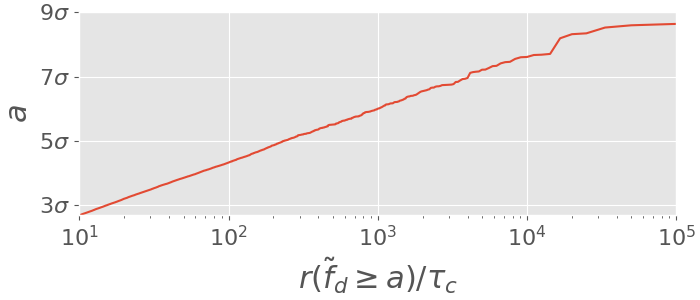
\includegraphics[width=.7\linewidth]{return_time/return_time.png}
	\caption{Amplitude of drag fluctuations as a function of the corresponding return time. $\tilde{f}_d$ denotes the drag with zero mean, \textit{i.e.} $\tilde{f}_d = f_d - \overline{f_d}$.
	}
	\label{fig:return_time_instant}
\end{figure}

% return time given from direct sampling
%
The phenomenology of extreme fluctuations of the drag is first investigated through brute-force direct sampling applied to the control run.
Direct sampling is here used as opposed to approaches involving rare-events algorithms discussed in section~\ref{sec:rare_events_algorithms}.
It will provide a trustworthy baseline for the validation of rare-events algorithms.

The waiting times $\tau$ are defined as the time between two consecutive occurrences of peak fluctuations with amplitude $f_d \geq a$, as illustrated in Fig.~\ref{fig:typical_drag_signal}.
The mixing time $\tau_m$ is the time needed for the dynamics to lose the memory of its initial condition.
As soon as the typical waiting times are much larger than the mixing time $\tau_m$, the occurrences of such events follow a Poisson process and the distribution of the waiting times is exponential, \emph{i.e.} $P(\tau)=\lambda(a)\exp(-\lambda(a)\tau)$ where $r(a)=1/\lambda(a)$ is the averaged waiting time \cite{lestang_computing_2018}; $r(a)$ is called the {\it return time} of the level $a$.
For systems without multi-stability, it is common for the mixing time $\tau_m$ to be of the order of the correlation time $\tau_c$.

How rare is a fluctuation $a$ is quantified by the return time $r(a)$.
We can define extreme drag fluctuations as \textit{rare events} in the sense that the return time is much larger than the correlation time, \emph{i.e.} $r(a) \gg \tau_c$.
%
%
If one assumes that  $r(a) = t(a)~/~\mathbb{P}(f_d\geq a)$   where the time scale $t(a)$ is of order $\tau_c$ and varies much more slowly with $a$ than ${\mathbb{P}(f_d\geq a)}$,
one might expect that
\begin{equation}
  \label{eq:return_time}
  r(a) \underset{a\to\infty}{\propto} \exp(la),
\end{equation}
where $l$ is the rate describing the positive tail of the \ac{pdf} of the drag (shown in Fig.~\ref{fig:pdf_drag}).
Fig.~\ref{fig:return_time_instant} shows the evolution of the return time $r(a)$ with the amplitude of fluctuation $a$, computed from {direct sampling} of the drag signal $f_d(t)$~\citep{lestang_computing_2018}.
Consistently, it is found that the return time $r(a)$ is well approximated by an exponential for large levels $a$. Let us also point out some deviation from the exponential law at the largest levels, which are probably the consequence of under-sampling.

% typically for $a \gtrsim 8 \sigma$ with $\sigma$ being the standard deviation.



\subsection{Extracting extreme drag fluctuations from a very long timeseries}
\label{sec:extreme_extraction}

% intro
%
We have extracted the fluctuations of the drag with a return time $r(a)$ greater than  $10^4\tau_c$ from the control time-series $\{f_d(t)\}_{0 \leq t \leq T_{tot}}$.
This set will be considered as representative of \emph{extreme events} in the upcoming study.
The choice of this particular threshold has been driven by the need to collect enough events with large amplitude and possibly identify generic features.
%
According to Fig.~\ref{fig:return_time_instant}, the related amplitude $a$ is found equal to $7.6~\sigma$ with $\sigma$ being the standard deviation of the drag process.
Precisely, 104 independent fluctuations with $f_d(t) \geq 7.6\sigma$ have been identified. Each fluctuation is characterized by its maximal value, $f_d^{\star}$, and the time, $t^{\star}$, at which this maximum is reached.
%
In the following, the phenomenology of extreme drag fluctuations will be examined on the basis of this set of events.

\subsection{Extreme fluctuations of the instantaneous drag}
\label{sec:instantaneous_drag}

\subsubsection{Contribution of forebody and base pressure fluctuations to the overall drag fluctuation}
\label{sec:forebody_and_base_contribution}

\begin{figure}
	\centering
	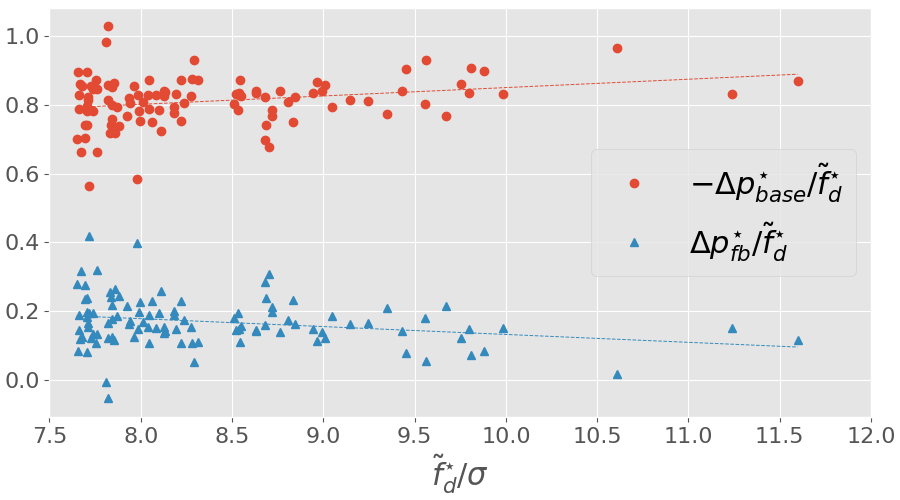
\includegraphics[width=.8\linewidth]{pressure_ratio/pressure_ratio.png}
	\caption{\label{fig:pressure_ratio} Relative contributions of the forebody and base pressure variations to extreme amplitudes of the drag. An extreme event corresponds to an amplitude $\tilde f^{\star}_d$ and a unique pair  ($\tilde{p}^{\star}_{base}$,~$\tilde{p}^{\star}_{fb}$).}
\end{figure}

% teasing
%
In section~\ref{sec:test_flow}, it was pointed out that drag fluctuations within one standard deviation were not associated with any particular arrangement of the vorticity around the obstacle.
In the following we show that the situation os different in the case of extreme drag fluctuations.

% relative contribution of forebody and base pressure
%
Let $(t^{\star}, f_d^{\star})$ refer to an extreme-drag event.
The (zero-mean) fluctuation $\tilde{f}_d^{\star} = f_d^{\star} - \overline{f_d}$ can be  decomposed into
\begin{equation}
\tilde{f}_d^{\star} = \Delta p_{fb}^{\star} - \Delta p_{base}^{\star}
\end{equation}
where $\Delta p_{fb}^{\star}$ and $\Delta p_{base}^{\star}$ denote the variations of the forebody and base pressure, respectively.
%
Fig.~\ref{fig:pressure_ratio} displays the relative contributions
$\Delta p_{fb}^{\star}/\tilde{f}_d^{\star}$ and $-\Delta p_{base}^{\star}/\tilde{f}_d^{\star}$ to the drag fluctuation $\tilde f_d^{\star}$.
It is found that very large fluctuations of the drag result mainly ($\sim 80\%$) from the drop of the base pressure, whereas the variation of forebody pressure contributes much less to $\tilde{f}_d^{\star}$.
On the contrary, moderate fluctuations arise from combined variations of the forebody and base pressures without any particular predominance, which is in agreement with the previous observations (see Fig.\ref{fig:typical_vorticity}).

\subsubsection{Fluid dynamics related to extreme drag fluctuations}
\label{sec:dynamical_aspects}

\begin{figure}
	\centering
	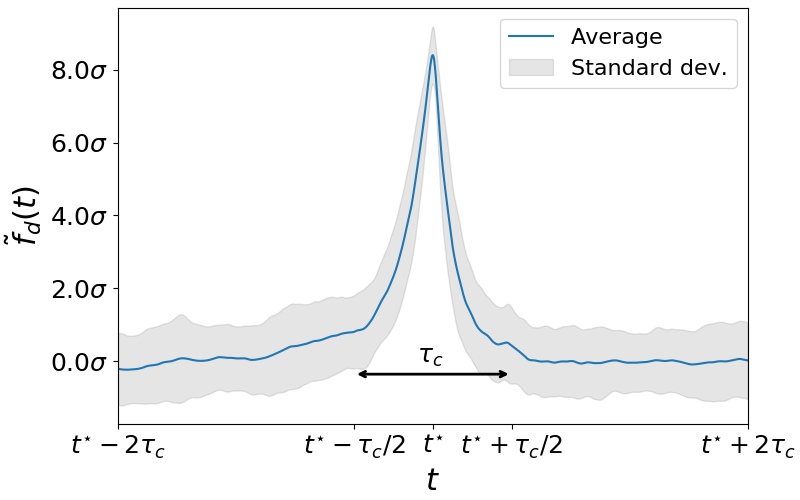
\includegraphics[width=.7\linewidth]{timeseries_extremes/timeseries_extremes.png}
	\caption{\label{fig:timeseries_extremes} Ensemble average of drag signals centred around extreme fluctuations occurring  at $t=t^{\star}$. The blue line shows the mean profile whereas the shaded area indicates variations (around the mean profile) within one standard deviation. Extreme-drag events exhibit a typical lifetime of one correlation time $\tau_c$. The profile is slightly skewed indicating that the step up is slower than the return to typical values.}
\end{figure}

% mean profile around burst
%
The focus is now on the flow scenarii that yield extreme values of the drag.
Fig.~\ref{fig:timeseries_extremes} displays the mean profile (in time) of the drag signal around extreme events. A peaked profile is observed with a width roughly corresponding to one correlation time $\tau_c$. This shows that the duration of extreme events corresponds typically to the sweeping time of the flow past the obstacle.
%Starting from typical values, extreme drags are typically reached in less than a correlation time.
Interestingly, the profile is also slightly skewed indicating that the step up of the drag is slower than the return to typical values past the peak value.
%This is reminiscent of time-irreversibility in turbulent dynamics.
This asymmetry (under time reversal) is closely linked to the symmetry breaking in what happens before and after the obstacle.
To better understand the flow scenarii leading to these events, the vorticity fields around the obstacle are now examined.

\begin{figure}
  \centering
  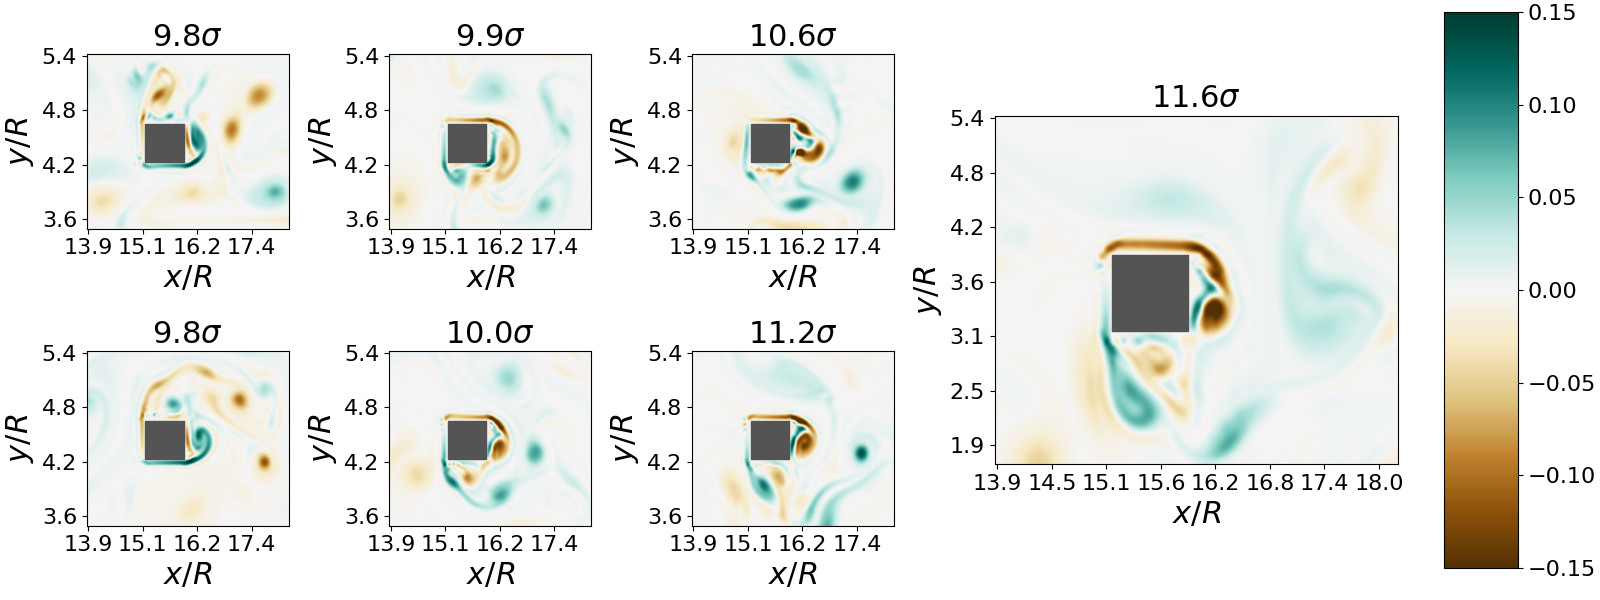
\includegraphics[width=\linewidth]{illustr_extrms_vorticity/illustr_extrms_vorticity.png}
  \caption{\label{fig:top_4_events_vorticity} Vorticity field (in lattice units) around the obstacle at $t=t^{\star}$ for the highest drag amplitudes recorded in the control run.
  }
\end{figure}

\begin{figure}
  \centering
  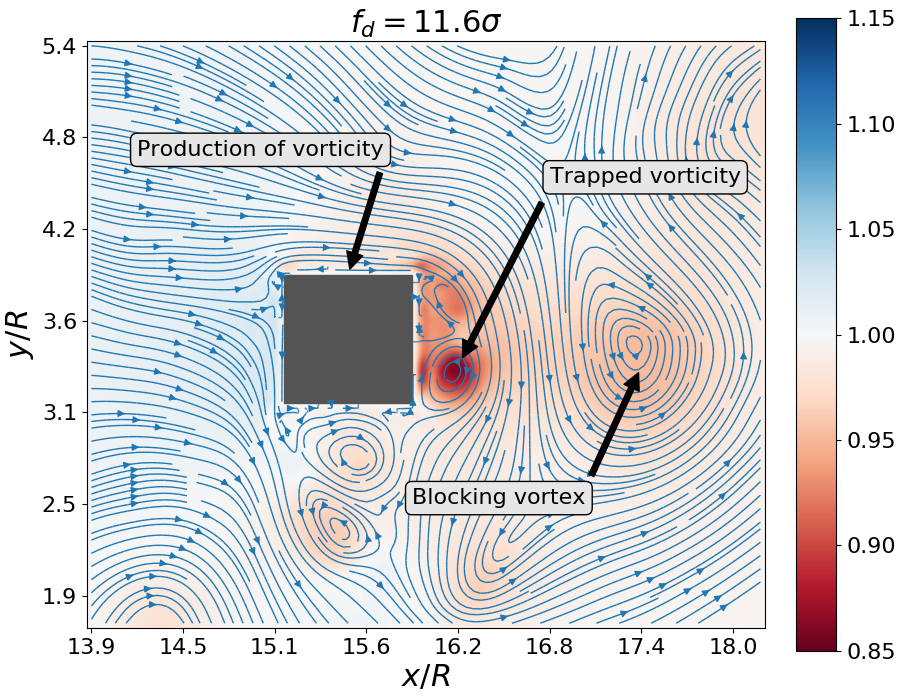
\includegraphics[width=.5\linewidth]{illustr_density_streamlines/illustr_density_streamlines.png}
  \caption{\label{fig:density+streamlines} Pressure field (in lattice units) and velocity streamlines at $t=t^{\star}$. In the near wake of the square, a (blocking) vortex blocks an intense vortex against the base of the obstacle.}
\end{figure}

\begin{figure}
  \centering
  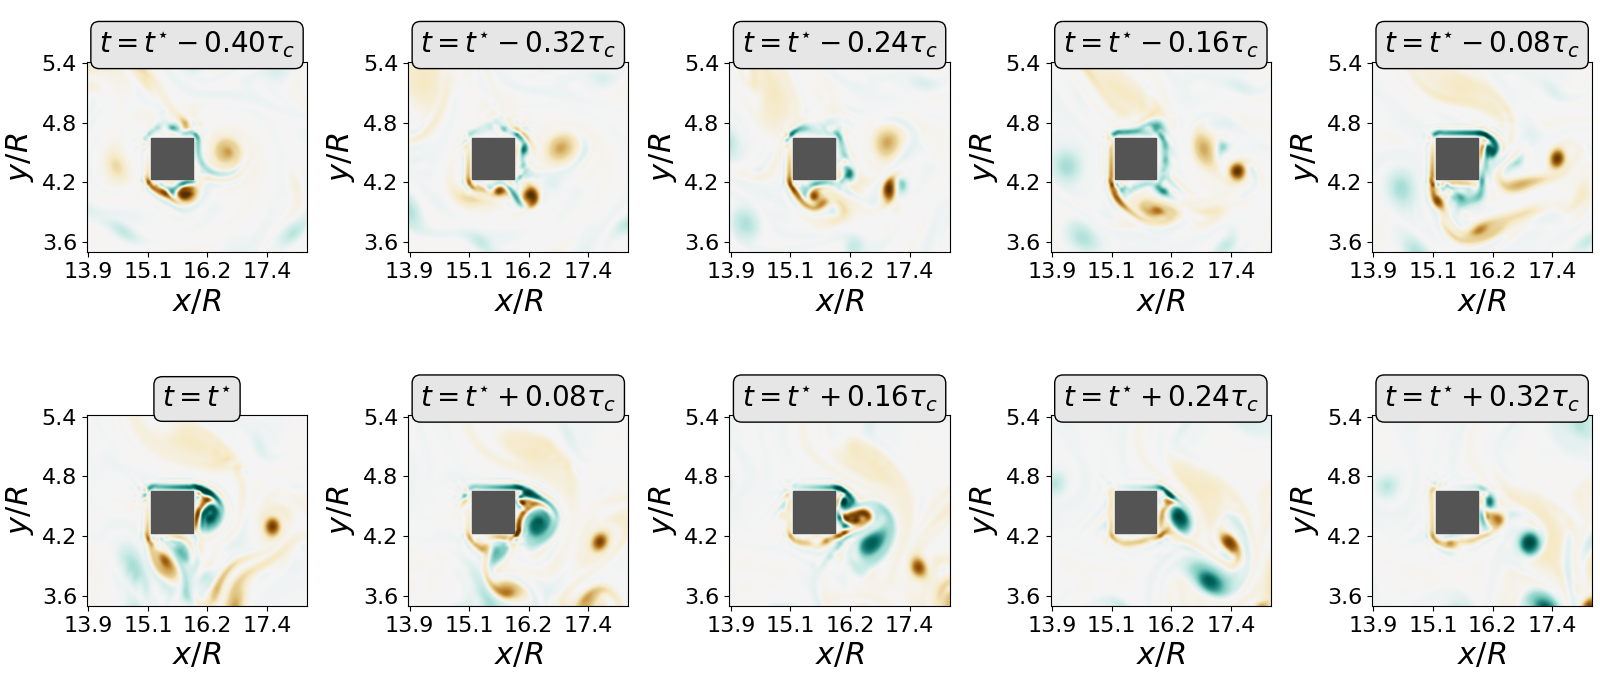
\includegraphics[width=.8\linewidth]{dynamics_extremes/dynamics_extremes.png}
  \caption{\label{fig:vorticity_dynamics} Snapshots of the vorticity field (in lattice units)  around $t=t^{\star}$.}
\end{figure}
% flow scenario
%
Fig.~\ref{fig:top_4_events_vorticity} displays the vorticity field (in lattice units) around the obstacle for the highest amplitudes of the drag during the control run.
%
In each case, an intense vortical structure is visible near the base of the obstacle.
The vorticity level of this structure is typically twice the amplitude of typical vorticity fluctuations observed in Fig.~\ref{fig:typical_vorticity}.
%+
The formation of this vortex originates from an intense negative (or positive) vorticity layer at the top (or bottom) boundary of the obstacle.
%
This high vorticity is responsible for a significant pressure drop at the base of the obstacle and therefore a strong drag.
In contrast, nothing special happens near the forebody of the obstacle during extreme-drag events.

The high pressure drop near the base of the obstacle appears to be closely related to the presence of a strong vortex blocked against the base.
As illustrated in Fig.~\ref{fig:density+streamlines}, this blockage is enforced by the presence of opposite vorticity in the near wake, which holds the vortex against the base of the obstacle and prevents it from being swept away for a while.
%
This scenario is better evidenced by Fig.~\ref{fig:vorticity_dynamics}, where the time history of the vorticity field around $t=t^\star$ for the same event is shown.
%
Before the occurrence of the extreme event, positive vorticity originating from the bottom boundary layer develops in the near wake of the square. This positive vorticity  prevents the shedding of negative vorticity and enforces the development of a intense vortex against the base of the square.
As the blocking vortex is in turn advected downstream, the vortex against the base is released.
%
Consistently, one can argue that the typical duration of this scenario is related to the sweeping time of the flow past the obstacle, and is therefore of the order of $\tau_c$.
This is in full agreement with the typical duration obtained from statistical consideration on the mean profile of large-drag fluctuations in Fig.~\ref{fig:timeseries_extremes}.
This scenario is generic and has been observed for most extreme events sampled in the control run.

%We found that $80\%$ of the extreme events sampled from the control timeseries can be related to very similar dynamics.

\begin{figure}
  \centering
  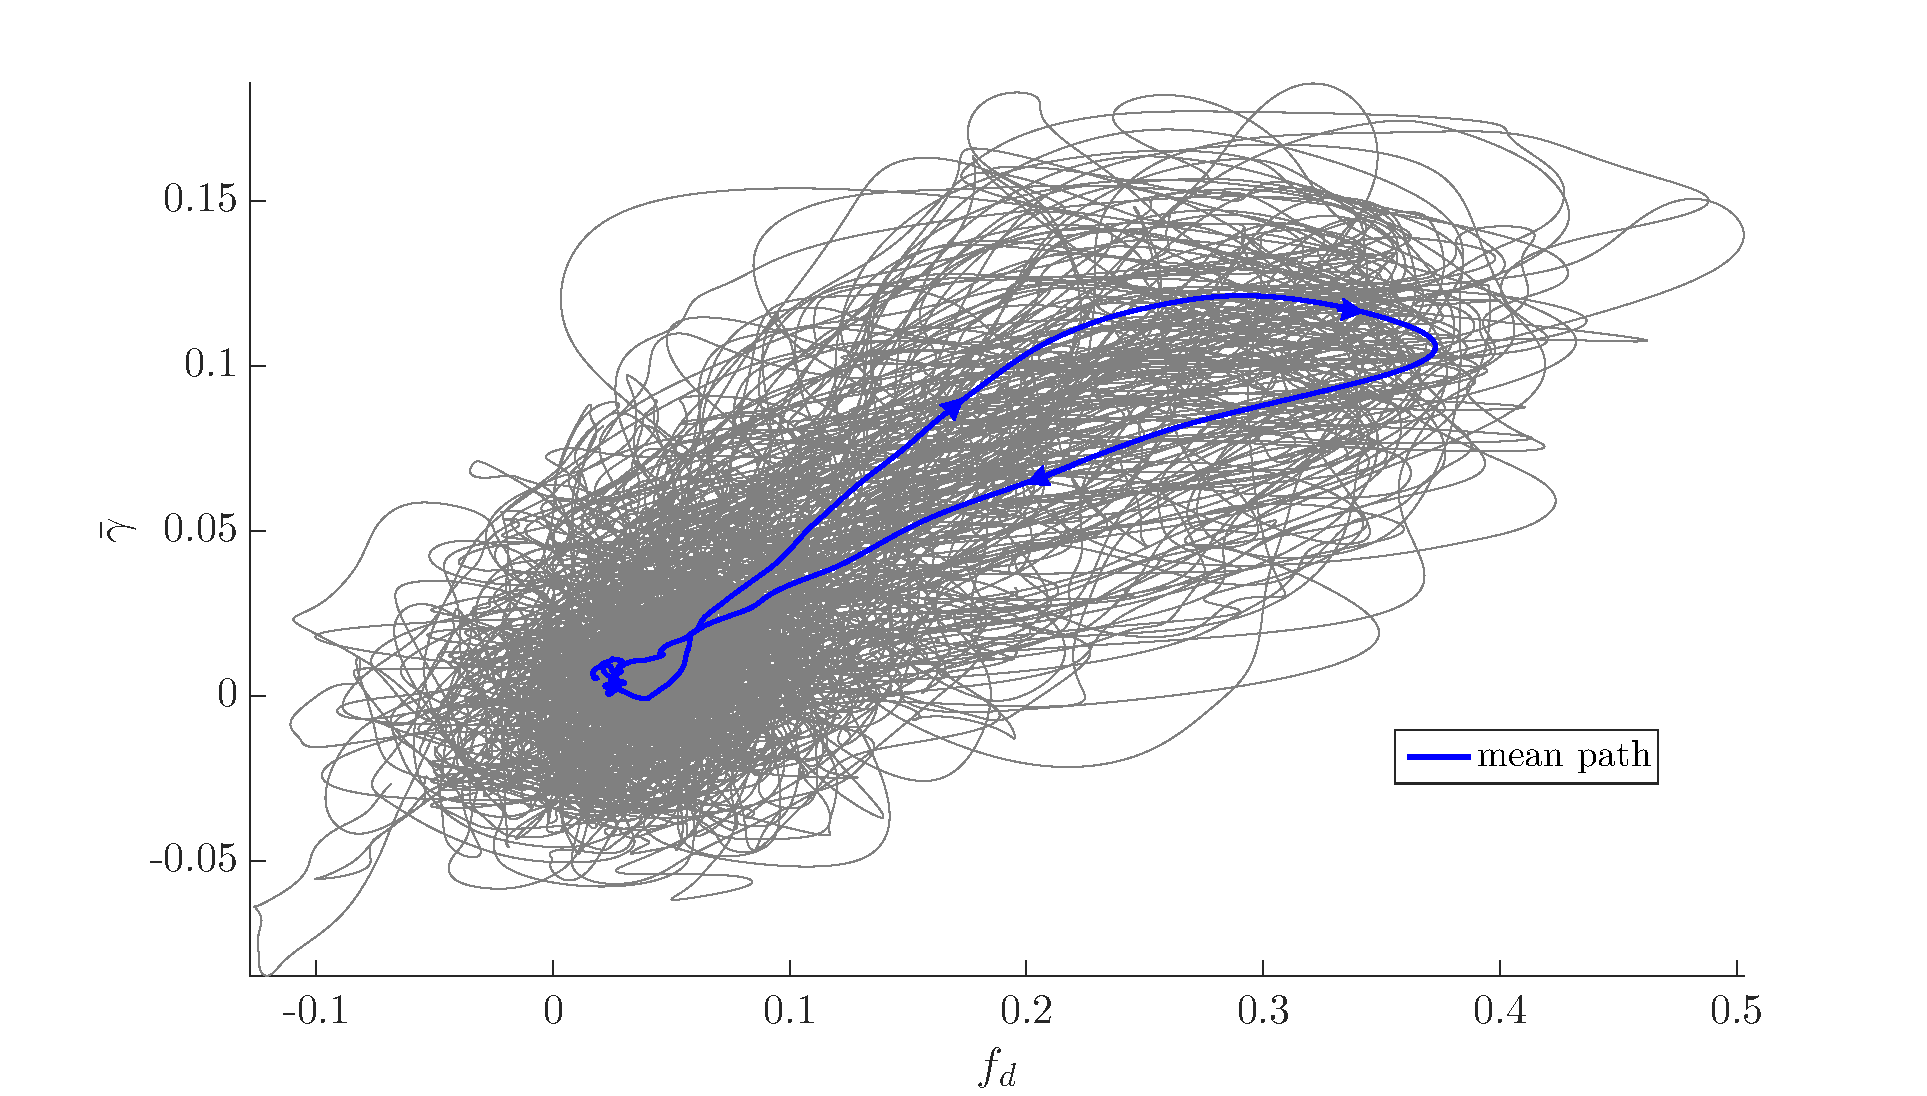
\includegraphics[width=.7\linewidth]{shear_asof_drag/shear_asof_drag}
  \caption{\label{fig:shear_asof_drag} Evolution of the (integrated) shear along the top or bottom sides of the obstacle as a function of the drag for $t^{\star}-2\tau_c \leq t \leq t^{\star}-2\tau_c$. Each trajectory corresponds to a single event. The blue line is the mean path averaged over the set of extreme events sampled in the control run.}
\end{figure}

Since the occurrence of large drag amplitudes arises from the production of vorticity along the top or bottom side of the square, it is proposed to characterize the dynamics of extreme events by their trajectory in the parameter space $(f_d(t), \bar{\gamma}(t))$ where $\bar{\gamma}(t)$ is the averaged shear along the top or bottom boundary of the square:
\begin{equation}
\label{eq:avg_shear_def}
\overline{\gamma} = \frac{1}{R} \int_{\mathcal{S}_\parallel} \frac{\partial u(\mathbf{x})}{\partial y}\mathrm{d}\mathbf{x},
\end{equation}
where $R$ denotes the size of the square, $u$ is the streamwise component of the velocity field and $\mathcal{S}_\parallel$ is the surface of either the top or the bottom boundary.
%
Fig.~\ref{fig:shear_asof_drag} shows $\overline{\gamma}(t)$ as a function of the instantaneous drag $f_d$(t) for $t^{\star}-2\tau_c \leq t \leq  t^{\star}+2\tau_c$ for the 104 sampled extreme events.
Before and after the extremal fluctuation, \textit{i.e.} for $t^{\star}-2\tau_c \leq t \leq t^{\star}-\tau_c$ and $t^{\star}+\tau_c \leq t \leq t^{\star}+2\tau_c$, paths wander in a region related to typical values of both $\overline{\gamma}$ and $f_d$.
On the contrary, the drag abruptly varies for $t^{\star}-\tau_c \leq t \leq t^{\star}+\tau_c$ near the extremal amplitude.
%Paths in the $(f_d, \bar{\gamma})$ space display excursions to atypical values for both $\bar{\gamma}$ and $f_d$.
These excursions always go clockwise, that is, $\overline{\gamma}$ attains its maximum value before $f_d$ does.
This is consistent with an increase of $\overline{\gamma}$ acting as a precursor for extreme drag fluctuations.
In this representation, we also observe that the path related to the increase of the drag is longer than the path related to the return to typical values.

\subsection{Extreme fluctuations of the time-averaged drag }
\label{sec:time_avg}

\begin{figure}
	\centering
	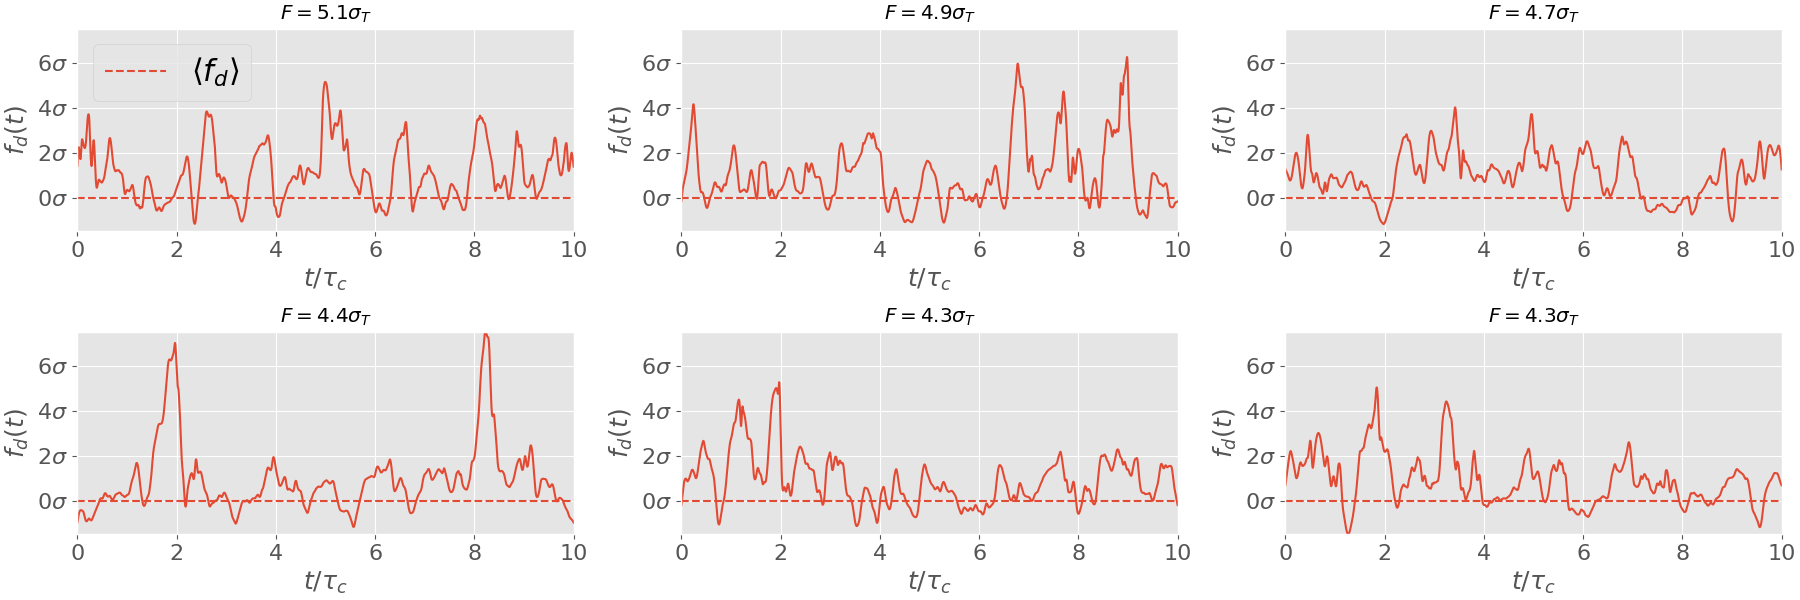
\includegraphics[width=\linewidth]{timeseries_extrms_AVG/timeseries_extrms_AVG}
	\caption{Instantaneous drag signals $f_d(t)$ corresponding to the highest fluctuations of the averaged  drag $F_T$ with a time window $T = 10 \tau_c$;  $\sigma$ and $\sigma_T$ denote the standard deviations of the instantaneous and averaged drag, respectively.}
	\label{fig:extreme_avg}
\end{figure}


% motivation
%
%In section~\ref{sec:instantaneous_drag}, we discussed the phenomenology of rare events corresponding to extremely high values of the drag acting on the square obstacle mounted in the flow described in section~\ref{sec:test_flow}. In particular, it was pointed out that such extreme drag fluctuations have a lifetime of, roughly, one correlation time $\tau_c$.

%We discussed previously the phenomenology of extreme fluctuations of the \emph{instantaneous} drag and pointed out that the time scale associated with the development of such event is of the order of the sweeping time of the flow past the obstacle $\tau_c$.
We discussed previously the phenomenology of extreme fluctuations of the \emph{instantaneous} drag, and identified the sweeping time of the flow past the obstacle as the characteristic lifetime of these events.
%
In applications, this duration may be much smaller than the response time of the material structure subject to these fluctuations, justifying a practical interest in the averaged (in time) drag force.
% Consider for instance the interaction of a deformable structure with a turbulent flow: the typical response time may be much larger than the lifetime of drag fluctuations.
%
% definition
%
Therefore, a relevant observable is the \textit{time-averaged} drag defined as
\begin{equation}
\label{eq:def_time_averaged_drag}
F_T(t) = \frac{1}{T}\int_t^{t+T} f_d(t) \mathrm{d}t,
\end{equation}
where $f_d(t)$ denotes the instantaneous drag and $T$ is the investigated timescale (response time).
In the following, we shall consider $T=10\tau_c$, where $\tau_c$ is the correlation of the instantaneous drag.
In that case, the PDF of $F_T$ is found nearly Gaussian as a consequence of the Central Limit theorem (see Fig.~\ref{fig:PDF_AVG}).
\begin{figure}
  \centering
  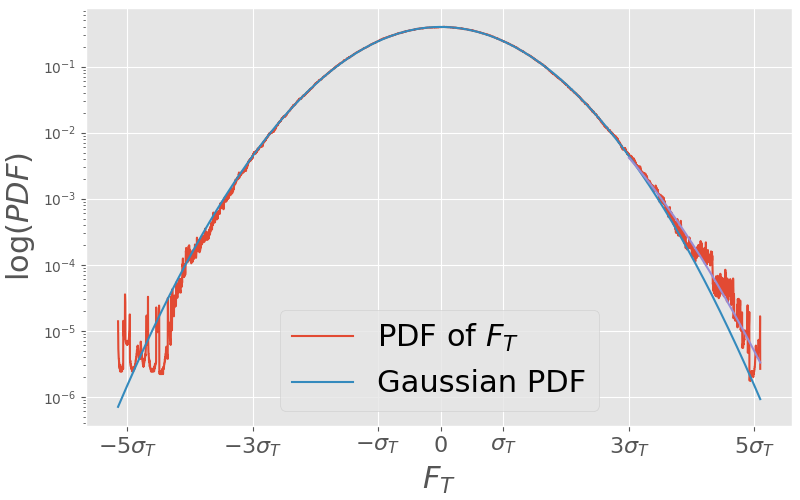
\includegraphics[width=.7\linewidth]{PDF_AVG/PDF_AVG}
  \caption{Estimate of the \ac{pdf} for the time-averaged drag $F_T$ with $T = 10\tau_c$. This estimate is based on a rolling average over a timeseries of the instantaneous drag $f_d$ of duration $4 \times 10^6 T_0$.}
    \label{fig:PDF_AVG}
\end{figure}

%
During a time interval $[t;t+T]$, a fluctuation of $F_T(t)$ may be roughly viewed as the overall contribution of  $T / \tau_c$ independent fluctuations of the {instantaneous} drag $f_d$.
% phenomenology
%
% What is the phenomenology leading to extreme values of $F_T(t)$ ?
It is thus legitimate to ask whether a large value of the averaged drag results from a single outstanding fluctuation of the instantaneous drag (case (1)),  or from  an unusual succession of moderate positive fluctuations (case (2)).
%
In the same way as in section \ref{sec:extreme_extraction}, one can identify extreme fluctuations of $F_T$ exceeding some fixed threshold $a$, and sample a set of extreme events.
By taking $a=5.2\sigma_T$ with $\sigma_T$ being the standard deviation of $F_T$, $84$ independent extreme events have been selected.
Again, this choice results from a compromise between the need to consider large deviations from the mean value and the requirement to sample a sufficient number of events for meaningful statistics. As a rule of thumb, the threshold has been set so that around one hundred events are selected.


% neither case (1) nor case (2)
%
Fig.~\ref{fig:extreme_avg} displays the time-series $\{f_d(t)\}_{t^{\star} \leq t \leq t^{\star}+T}$ for several extreme fluctuations of $F_T$ occurring at $t=t^\star$.
Qualitatively, it is found that extreme fluctuations of the time-averaged drag can neither be reduced to case (1) nor case (2).
Indeed, both cases are %equally
featured in Fig.~\ref{fig:extreme_avg};
very large value of the averaged-drag appear to result from either a very large fluctuation, or a significant succession of moderate (positive) fluctuations of the instantaneous drag.

%%% Local Variables:
%%% mode: latex
%%% TeX-master: "draft_p2_jfm"
%%% End: